\chapter{System Design}

\section{System Overview}

WattMate is a portable measurement system designed to monitor the behavior of power banks during both charging and discharging conditions. The system is inserted inline between a power source and a load, allowing continuous monitoring of current and voltage, without interrupting normal operation.

The main purpose of the system is to provide accurate and real-time measurements of portable energy storage devices that supports the USB Power Delivery (PD) standard. Measured data are processed by a microcontroller and are made available locally, using a display, and remotely through Bluetooth Low Energy (BLE) communication, enabling both real-time visualization and analysis through a mobile application.

The system is optimized for low-power operation, compact integration, and bidirectional power flow measurement, enabling analysis of both input charging conditions and output discharge performance.

At this stage, the system is designed to operate exclusively as a standalone module externally connected to a power bank. However, several measurement and monitoring features have already been implemented to ensure future scalability. In particular, the architecture has been designed to allow the PCB to be easily adapted, with minimal redesign effort, for integration with a battery management system (BMS) directly inside an energy storage device.

\subsection{System Objectives}\label{system_objectives}

The system is designed to achieve the following objectives:

\begin{itemize}
    \item Enable real-time monitoring of the power bank parameters including voltage and current.
    
    \item Ensure accurate and reliable measurements across the specified operating conditions and environment.
    
    \item Support high power levels, ensure compatibility with USB Power Delivery (PD) 3.1 140W devices.
    
    \item Provide derived diagnostics such as power estimation, energy consumption, battery State of Charge (SoC), battery State of Health (SoH) and cycle count.

    \item Ensure safe inline operation between source and load with appropriate power handling and thermal constraints.

    \item Enable wireless access to system data via BLE for external visualization and monitoring.
    
    \item Provide a user-friendly interface for local interaction and data visualization.
    
    \item Ensure manufacturability and serviceability through appropriate component selection and design for assembly.

    \item Provide a compact and portable solution suitable for embedded and battery-powered operation.
    
    \item Enable, with minimal redesign effort, future integration of the PCB with a battery management system (BMS) directly inside an energy storage device.
    
    \item Enable the future integrated system to measure battery pack temperature to provide thermal supervision of the power bank.

\end{itemize}

\subsection{System Scope}

The project delivers a fully functioning system for measurement, processing, communication, and user interaction, complemented by a mobile application for data visualization and interaction with the embedded system via BLE.

\textbf{Included in Scope:}
\begin{itemize}
    \item \textbf{Embedded hardware (PCB):} Design and implementation of the measurement, power management, and communication hardware, including current, voltage and temperature sensing circuits, power path routing, and BLE antenna integration.

    \item \textbf{Embedded firmware:} Implementation of data acquisition, signal processing, system control, data display and wireless communication.

    \item \textbf{Communication protocol:} Definition and implementation of BLE services for data exchange.

    \item \textbf{Mobile application:} Application for data visualization and interaction with the embedded system via BLE.

    \item \textbf{Mechanical design:} Design of the enclosure and mounting system.
\end{itemize}

\textbf{Excluded from Scope:} 
\begin{itemize}
    \item The system does not operate as a BMS and is not capable of actively interrupting or managing the power flow.
    \item The integration of a BMS is intended as a future feature and is not included in the current design revision.
    \item The system does not participate in the USB Power Delivery (PD) 3.1 negotiation process. It operates as a passive pass-through device and does not modify or interfere with the PD communication stack. 
    \item Compatibility is limited to USB PD 3.1 power levels up to 140 W.
    \item The system is not intended to function as a standalone power source or energy storage unit.
\end{itemize}

\newpage
\section{System Requirements}\label{sec:system_requirements}

\begin{longtable}{@{} L{1cm} L{1.5cm} L{12.5cm} @{} }
%\toprule
\headerrow
%\midrule
\addlinespace
\endfirsthead

%\toprule
\headerrow
%\midrule
\addlinespace
\endhead

%\midrule
\addlinespace
\multicolumn{3}{r}{\small\itshape Continued on next page}
\endfoot

%\bottomrule
\endlastfoot

%========================================================
% MEASUREMENT AND SENSING REQUIREMENTS
%========================================================

\categoryrow{\Req{req:measurement}}{Measurement and Sensing Requirements}
\addlinespace

%---------------- Voltage ----------------
\requirementrow{\ReqSub{req:measurement-voltage}}{Voltage}
\addlinespace

HW & \ReqSubSub{req:volt_table} &
The system shall support the following USB Power Delivery 3.1 voltage levels:

\vspace{0.3cm}

\noindent\begin{tabular}{c c c c c c}
    \toprule
    \textbf{V Nom} &
    \textbf{V Min} &
    \textbf{V Max} &
    \textbf{I Nom} &
    \textbf{Power} &
    \textbf{Supported} \\
    \midrule

    \SI{5}{\volt}  & \SI{4.75}{\volt}  & \SI{5.25}{\volt}  & \SI{3}{\ampere} & \SI{15}{\watt} & Yes \\
    \SI{9}{\volt}  & \SI{8.55}{\volt}  & \SI{9.45}{\volt}  & \SI{3}{\ampere} & \SI{27}{\watt} & Yes \\
    \SI{15}{\volt} & \SI{14.25}{\volt} & \SI{15.75}{\volt} & \SI{3}{\ampere} & \SI{45}{\watt} & Yes \\
    \SI{20}{\volt} & \SI{19}{\volt}    & \SI{21}{\volt}    & \SI{5}{\ampere} & \SI{100}{\watt} & Yes \\
    \SI{28}{\volt} & \SI{26.6}{\volt}  & \SI{29.4}{\volt}  & \SI{5}{\ampere} & \SI{140}{\watt} & Yes \\
    \SI{36}{\volt} & \SI{34.2}{\volt}  & \SI{37.8}{\volt}  & \SI{5}{\ampere} & \SI{180}{\watt} & No \\
    \SI{48}{\volt} & \SI{45.6}{\volt}  & \SI{50.4}{\volt}  & \SI{5}{\ampere} & \SI{240}{\watt} & No \\

\end{tabular}
\\
\midrule

HW & \ReqSubSub{req:volt_nominal} &
The system shall measure nominal bus voltage within the 5 V to 28 V operating range. Supported voltage levels are compliant with a subset of the USB Power Delivery 3.1 specification up to 140W, as defined in~\ref{req:volt_table}.\\
\midrule

HW & \ReqSubSub{req:volt_rating} &
The system shall withstand input voltages within $\pm 5\%$ of each supported nominal voltage level without degradation or damage.\\
\midrule

HW & \ReqSubSub{req:volt_acc} &
Voltage measurement error shall not exceed $\pm\SI{1}{\percent}$ of reading over the operating range.\\



%---------------- Current ----------------
\addlinespace
\requirementrow{\ReqSub{req:measurement-current}}{Current}
\addlinespace

FW & \ReqSubSub{req:curr_rating} &
The system shall support and measure bidirectional current up to $\SI{5}{\ampere}$ between source and load, covering all supported power levels defined in~\ref{req:volt_table}.\\
\midrule

FW & \ReqSubSub{req:curr_min} &
The system shall measure bidirectional current down to $\pm\SI{100}{\milli\ampere}$ ensuring an accuracy meeting the specified by~\ref{req:curr_acc}.\\
\midrule

FW & \ReqSubSub{req:curr_acc} &
Current measurement error shall not exceed $\pm\SI{1}{\percent}$ of reading over the operating range.\\



%---------------- Power ----------------
\addlinespace
\requirementrow{\ReqSub{req:power}}{Power}
\addlinespace

HW & \ReqSubSub{req:pow_rating} &
The system shall measure bidirectional power up to $\pm\SI{140}{\watt}$.\\
\midrule

HW & \ReqSubSub{req:pow_acc} &
Power measurement error shall not exceed $\pm\SI{2}{\percent}$ of reading over the operating range.\\



%---------------- Temperature ----------------
\addlinespace
\requirementrow{\ReqSub{req:measurement-temperature}}{Temperature}
\addlinespace

HW & \ReqSubSub{req:temp_rating} &
The system shall support temperature measurement over the operating range from $\SI{-20}{\celsius}$ to $\SI{85}{\celsius}$ under normal operating conditions.\\
\midrule

HW & \ReqSubSub{req:temp_acc} &
Temperature measurement error shall not exceed $\pm\SI{1}{\celsius}$ over the full operating temperature range.\\



%---------------- Sampling ----------------
\addlinespace
\requirementrow{\ReqSub{req:measurement-sampling}}{Sampling}
\addlinespace

HW FW & \ReqSubSub{req:perf_sampling} &
The system shall acquire electrical signals with a sampling period not exceeding $\SI{20}{\milli\second}$ ($\SI{50}{\hertz}$) during ON-state operation.\\
\midrule

FW & \ReqSubSub{req:perf_lowpower} &
Sampling periods greater than $\SI{20}{\milli\second}$ are permitted when no power flow is detected and the system operates in low-power mode.\\




%========================================================
% POWER REQUIREMENTS
%========================================================
\addlinespace
\categoryrow{\Req{req:power}}{Power Requirements}
\addlinespace

\requirementrow{\ReqSub{req:power-delivery}}{Power Delivery Protocol}
\addlinespace

HW & \ReqSubSub{req:inline_op} &
The system shall operate inline between a power source and a load without interrupting power delivery.\\
\midrule

HW & \ReqSubSub{req:inline_pd} &
The system shall not interfere with the USB Power Delivery negotiation process.\\


\addlinespace
\requirementrow{\ReqSub{req:power-consumption}}{Power Consumption}
\addlinespace

HW FW & \ReqSubSub{req:pwr_consumption} &
The system shall limit internal power consumption to preserve battery life and maintain efficient operation.\\
\midrule

HW FW & \ReqSubSub{req:pwr_efficiency} &
ON-State efficiency shall be greater than or equal to $\SI{99}{\percent}$ under worst operating conditions.\\
\midrule

HW FW & \ReqSubSub{req:pwr_battery} &
OFF-State battery life shall be at least $\SI{1}{year}$ when using a power bank with $\SI{32}{\watt\hour}$ of stored energy.\\




%========================================================
% SAFETY REQUIREMENTS
%========================================================
\addlinespace
\categoryrow{\Req{req:safety}}{Safety Requirements}
\addlinespace

\requirementrow{\ReqSub{req:safety-electrical}}{Electrical Fault Detection}
\addlinespace

HW FW& \ReqSubSub{req:over_alert} &
The system shall detect over-voltage and over-current conditions and notify the user through an alert message.\\
\midrule

HW FW& \ReqSubSub{req:under_alert} &
The system shall detect under-voltage condition and notify the user through an alert message.\\


\addlinespace
\requirementrow{\ReqSub{req:safety-thermal}}{Thermal Fault Detection}
\addlinespace

HW FW& \ReqSubSub{req:thermal_fault} &
The system shall detect over-temperature condition and notify the user through an alert.\\



%========================================================
% PROCESSING AND COMMUNICATION
%========================================================
\addlinespace
\categoryrow{\Req{req:processing}}{Processing and Communication Requirements}
\addlinespace

\requirementrow{\ReqSub{req:processing-data}}{Data Processing}
\addlinespace

HW & \ReqSubSub{req:mcu} &
The system shall include a microcontroller unit (MCU) selected between the available options of the Texas Instruments CC2640R2F family.\\
\midrule

FW & \ReqSubSub{req:data_proc} &
The system shall process raw sensor data and compute derived electrical quantities such as energy, SoC, and SoH.\\


\addlinespace
\requirementrow{\ReqSub{req:processing-ble}}{Bluetooth Low Energy}
\addlinespace

HW FW& \ReqSubSub{req:ble_tx} &
The system shall transmit measured and computed data to an external device via Bluetooth Low Energy (BLE).\\



%========================================================
% INTERFACE REQUIREMENTS
%========================================================
\addlinespace
\categoryrow{\Req{req:interface}}{Interface Requirements}
\addlinespace

\requirementrow{\ReqSub{req:interface-display}}{Display}
\addlinespace

HW FW& \ReqSubSub{req:ui_display} &
The system shall provide local visualization of measurements through an integrated display.\\


\addlinespace
\requirementrow{\ReqSub{req:interface-input}}{Input}
\addlinespace

HW FW& \ReqSubSub{req:ui_buttons} &
The system shall allow basic user interaction through physical input buttons.\\


%========================================================
% MANUFACTURING AND SERVICE
%========================================================
\addlinespace
\categoryrow{\Req{req:manufacturing}}{Manufacturing and Service}
\addlinespace

\requirementrow{\ReqSub{req:manufacturing-assembly}}{Assembly}
\addlinespace

HW & \ReqSubSub{req:assembly} &
The electronic component packages of the system shall be selected to allow, whenever feasible, manual placement and soldering without requiring fully automated manufacturing tools.\\
\midrule

HW & \ReqSubSub{req:passives} &
Passive components shall use packages not smaller than 0603 (imperial units).\\
\midrule

HW & \ReqSubSub{req:packages} &
Package selection shall not compromise system performance or prevent compliance with any other system requirement.\\

\addlinespace
\requirementrow{\ReqSub{req:manufacturing-service}}{Programming and Serviceability}
\addlinespace

HW & \ReqSubSub{req:reprogramming} &
The system firmware shall be fully reprogrammable through a JTAG interface. The programming connector shall remain accessible after opening the system enclosure without requiring PCB removal.\\
\midrule

%========================================================
% ENVIRONMENT
%========================================================
\addlinespace
\categoryrow{\Req{req:operating-environment}}{Operating Environment}
\addlinespace

\requirementrow{\ReqSub{req:environmental-conditions}}{Environmental Conditions}
\addlinespace

HW & \ReqSubSub{req:operating-temperature-range} &
The system shall operate reliably within an ambient temperature range from $\SI{-20}{\celsius}$ to $\SI{85}{\celsius}$, compatible with typical consumer and automotive-adjacent environments. \\
\midrule

HW & \ReqSubSub{req:humidity-resistance} &
The system shall tolerate non-condensing humidity levels encountered in standard indoor and light outdoor operating conditions without degradation of electrical performance or measurement accuracy. \\
\midrule

HW & \ReqSubSub{req:vibration-and-mechanical-stress} &
The PCB assembly and mounted components shall be designed to withstand moderate mechanical vibration and handling stress typical of portable embedded systems, without electrical discontinuities or solder joint failures. \\
\midrule


%========================================================
% EXPANDIBILITY
%========================================================
\addlinespace
\categoryrow{\Req{req:future-expandability}}{Future Expandability}
\addlinespace

\requirementrow{\ReqSub{req:bms-integration}}{BMS Integration}
\addlinespace

HW & \ReqSubSub{req:no-active-bms} &
The system shall not implement Battery Management System functionality in the current revision and shall not actively interrupt, regulate, or control the power flow between source and load. \\
\midrule

HW & \ReqSubSub{req:modular-measurement-extension} &
The measurement and sensing subsystem shall be implemented in a modular way, allowing future extension for internal energy storage integration with minimal modification to the existing PCB and circuitry. \\
\midrule

HW & \ReqSubSub{req:temperature-sensing-flexibility} &
The temperature sensor placement shall allow optional removal or unsoldering without impacting core system functionality, and shall be positioned such that it can be extended beyond the PCB boundary in future revisions to ensure direct thermal contact with battery cells. \\
\midrule

\end{longtable}


\newpage
\section{System Architecture}

\subsection{Architecture Overview}

The system is designed as an external power monitoring device intended to operate between a USB-C power source and a connected load. The main power path connects the USB-C input connector directly to the USB-C output connector, allowing energy transfer without actively participating in the USB Power Delivery negotiation process.

Electrical quantities are acquired through a dedicated power sensing stage inserted in the power path. The sensor continuously monitors voltage and current and communicates the acquired measurements to the microcontroller unit (MCU) through a serial interface.

The MCU represents the central control and processing element of the architecture. Its responsibilities include sensor acquisition, computation of derived quantities, execution of application logic, system supervision, user interface management, and wireless communication handling.

Local user interaction is provided through an integrated display and one physical input button. The display provides real-time visualization of measured and computed data, while the button allow user navigation and interaction with system functions.

Temperature monitoring is implemented using a sensing element connected to the MCU to provide future thermal supervision of the power bank while supporting other diagnostic functionality such as SoH.

Power required by the embedded electronics is generated through a dedicated DC-DC conversion stage that derives regulated supply rails independently from the monitored USB bus voltage. This allows stable operation of the digital and analog subsystems across the supported input voltage range.

Wireless connectivity is enabled through the MCU integrated RF interface and a pcb integrated antenna, allowing external devices to access measurement data, system status information, and telemetry through Bluetooth Low Energy (BLE).

Overall, the proposed architecture separates power transfer, measurement, processing, communication, and user interaction functions into dedicated subsystems to improve modularity, simplify validation activities. The system design also includes architectural decisions intended to support future system evolution. Although the current implementation operates as an external inline measurement platform, several subsystems were intentionally designed to be reusable in future embedded battery-management applications. Examples include the external temperature sensing interface and battery-state estimation capabilities.

\newpage
\subsection{Block Diagram}

Figure~\ref{fig:block_diagram} shows the functional decomposition of the system and the interactions between the main subsystems. The diagram represents the data, power, and control relationships between functional blocks rather than the physical implementation.

\begin{figure}[H]
    \centering
    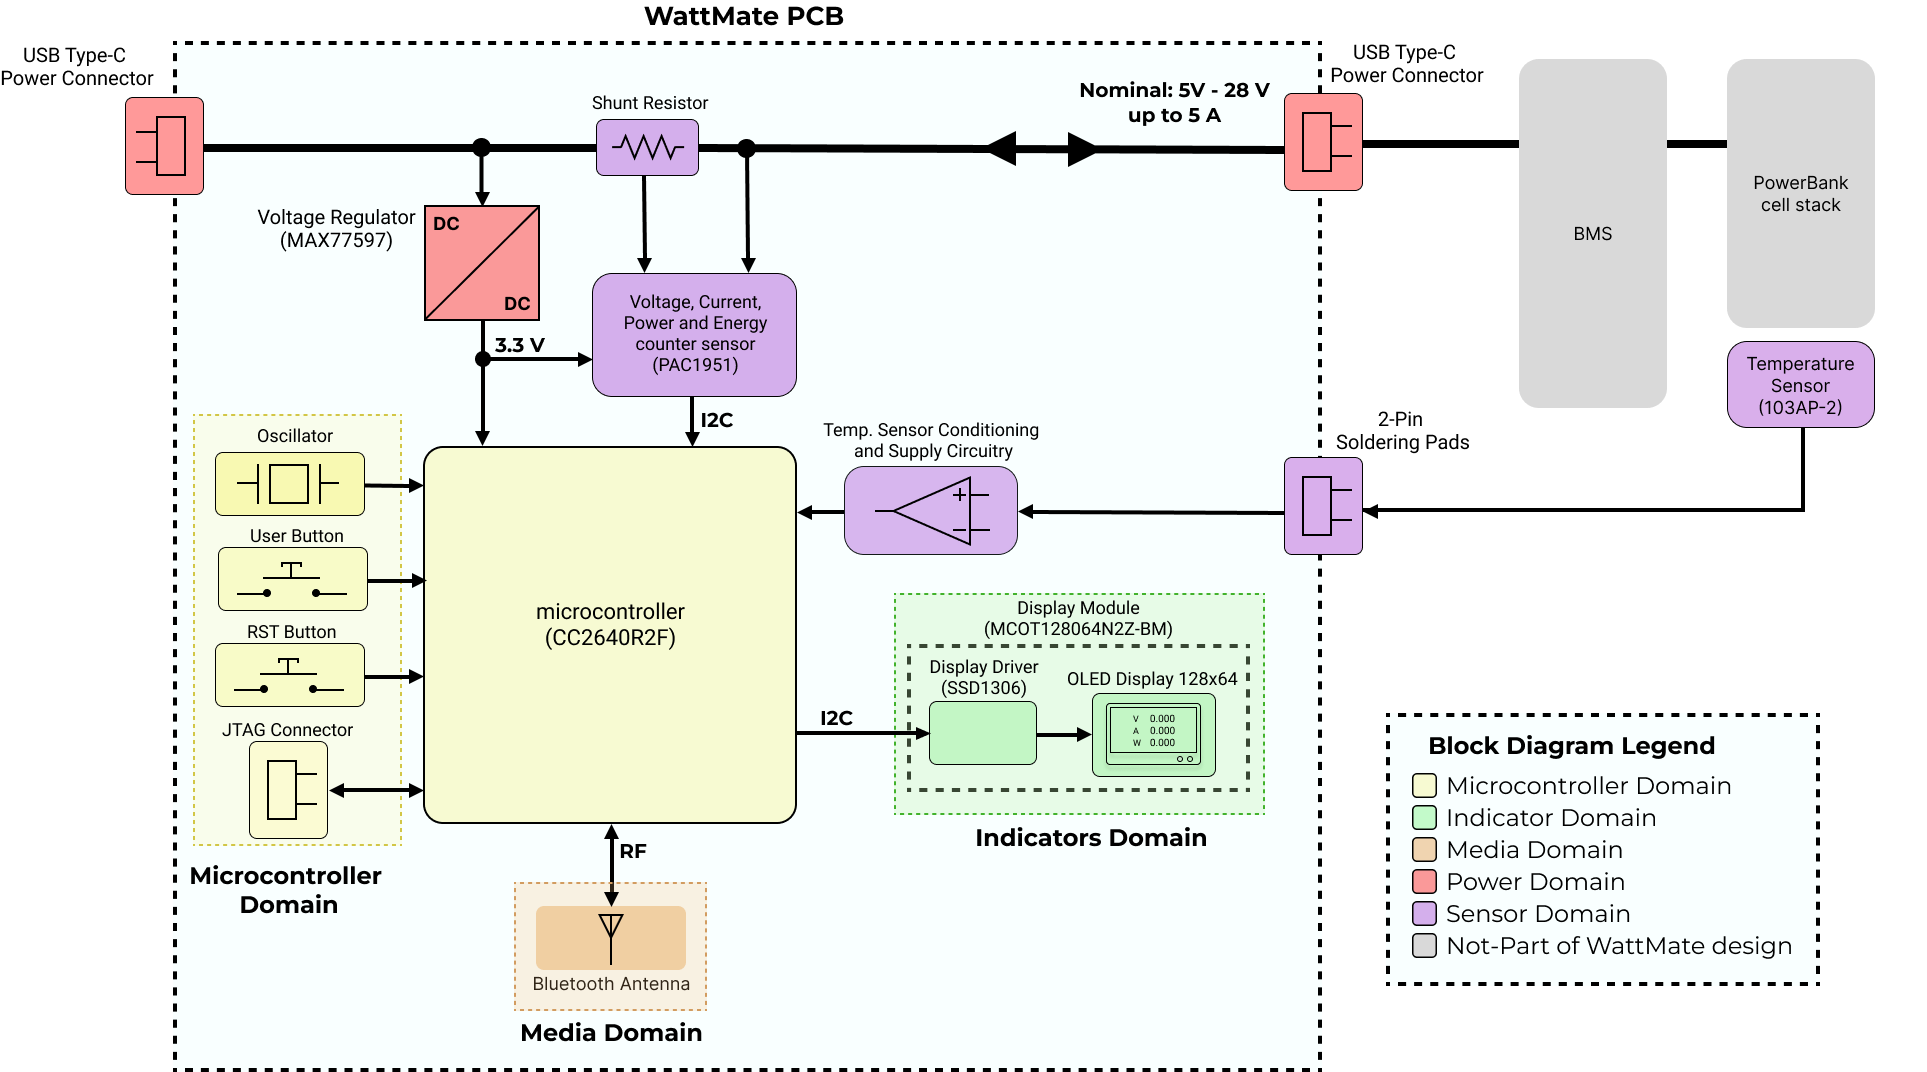
\includegraphics[width=1.0\linewidth]{figures/1_SYS_figures/block_diagram.png}
    \caption{System block diagram showing functional architecture and interconnection between subsystems.}
    \label{fig:block_diagram}
\end{figure}


\subsubsection{Power Connectors and DC Bus}

The main power path, hereafter referred to as the DC bus, represents the primary energy transfer path within the system. It is interrupted by the current sensing element and connects the DC input port to the DC output port. The DC input port is defined as the port always connected to the power bank or battery pack, while the DC output port is defined as the port that, during the discharge phase, is connected to the load. This nomenclature is fixed and is consistently maintained even during the charging phase of the power bank or battery pack.

\subsubsection{Electrical Measurement}

This subsystem performs monitoring of the DC bus electrical quantities, which are then transmitted to the MCU for further analysis and display. In order to save space on the board and keep connection complexity low, measured data are transmitted through a serial communication interface, reducing the number of required signal lines. This subsystem is also responsible for the alert generation, which shall operate according to the safety requirement~\ref{req:over_alert}.

\subsubsection{Temperature Measurement}

A temperature sensing circuit is also included in the prototype. In the current version of WattMate, the sensor can not be directly attached to any battery cells, since the device is implemented as an external inline monitor. However, this functionality was included to validate a sensing approach that could become relevant in future versions of the system, especially in the case of direct integration into the electronics of a battery pack or power bank, as described in Section~\ref{system_objectives}. 

This subsystem performs monitoring of the battery pack temperature, which is then transmitted to the MCU for further analysis and display. In the future integrated system, proper measurement of the battery pack temperature requires the sensor to be placed in direct thermal contact with the cells, which is not feasible if the sensing element is fixed on the main PCB. For this reason, the temperature sensor is connected to the system through wires or metal leads, allowing flexible placement of the sensing element while keeping the main board compact and electrically unchanged.

\subsubsection{RF Communication}

The RF communication subsystem enables wireless data exchange between WattMate and external devices through Bluetooth Low Energy (BLE), providing access to measurement data and system status information. To maintain a compact and cost-effective design the RF interface is integrated directly within the system architecture, avoiding the need for an external antenna. This approach is compatible with the required short-range communication typical of BLE applications.

\subsubsection{User Interface}

The user interface subsystem provides local interaction between the user and the system. Through an integrated display, it presents all measured and computed quantities, as well as system status information and fault or alarm conditions.
As for the other subsytems, data transfer between the MCU and the display is implemented through a serial communication interface, in order to keep connection complexity low.
This subsystem also captures user input through a physical button and forwards it to the MCU for handling display navigation and system control operations.


\subsubsection{MCU}

The MCU represents the central coordination element of the overall system. It is responsible for acquiring data from the sensor and user input subsystems and coordinating their operation to implement the required timing behavior.

The acquired data are processed by the MCU to compute derived quantities such as power, energy, State of Charge (SoC), and State of Health (SoH). These results are made locally available to the user through the display. The MCU also manages the BLE communication, which is implemented with a bidirectional channel, allowing the system to receive commands and data from external devices as well as transmit measurement data and telemetry information.

The MCU also supervises and controls all previously mentioned subsystems to ensure correct system operation while optimizing overall power consumption. This contributes to maximizing battery life by dynamically managing system resources based on operational needs.



\subsubsection{Power Supply}

The power supply subsystem generates and regulates the internal voltage rail required for the operation of all the subsystems. It ensures correct operation under varying input conditions by deriving a stable supply by stepping down the power bank provided voltage.

The power supply is powered from the output connector side of the system in order to achieve accurate estimation of the power bank capacity. In this configuration, during a charging cycle, WattMate measures only the current flowing into the battery pack, excluding the contribution of the system's own consumption. Since the system consumption cannot be easily measured and compensated for, this architectural choice enables accurate capacity estimation without the need for additional sensing circuitry.
